\documentclass[10pt,a4paper,tikz]{article}
\usepackage[utf8]{inputenc}
\usepackage{amsmath}
\usepackage{amsfonts}
\usepackage{amssymb}
\usepackage{pgf}
\usepackage{comment}
\author{Paul Kline}
\begin{document}
\title{Measurement Deadlock Resolution}

\maketitle

In measurement rule based remote attestation, both the attester and appraiser have Privacy Policy rules. These rules could easily result in a measurement deadlock. \\

For example, let's say we are entity \textit{A} acting as the appraiser, and we wish to know that entity \textit{B} is running an approved virus checker (if any). Additionally, \textit{B} has a privacy policy rule that says \textit{B} will not reveal the status of a virus checker to anyone without knowing that the requesting entity is running an approved operating system. However unfortunately, \textit{A} has a Privacy Policy rule that says \textit{A} will not reveal its operating system to anyone without first knowing they are running an approved virus checker. We have now entered a state of Measurement Deadlock. The rest of this paper addresses how this can be handled. \\

One way is to require the protocol writer to include `compromises' in the definition of each rule. This of course results  in a much more complex set of rules, not to mention the writer is required to make compromises to their Privacy Policy. For example, \\

\textbf{Reveal} OS \textit{if} VC known \& OK \\
becomes 

\textbf{Reveal} OS \textit{if} VC known \& OK \\
\textit{Case} Deadlock \\
\textbf{Compromise} \textit{if} \dots \\
\textit{try} \dots \\
\textit{try} \dots \\
\vdots 

Even with such complex rules it would be difficult or perhaps impossible to get the behavior desired and expected. Now we have to record when compromises were made and potentially make future Privacy Policy decisions based on the compromise. Plus we have made rule writing exponentially more difficult for the protocol writer. In every way, compromises are awful. This reminds me a joke. My wife wanted a cat. I wanted a dog. So we compromised and got a cat. 
\\

Another way the appraiser could handle such a deadlock would be to simply reject further communication with the entity. Perhaps this is the desired behavior in some situations when the attitude is \textit{``if you won't give me the measurement, fine then. We're done here; your loss"}. This has the benefit that this method involves no compromises having to be written nor executed. Essentially we have ``assumed the worst" by interpreting no measurement as a bad measurement. 

However, often times it would be useful to continue the attestation process. But we don't want to require anyone to make compromises to their Privacy Policy (we want to have our cake and eat it too). This is more than a ``I'll show you mine if you show me yours at the count of 3" problem. Not only do we want to simultaneously trade measurements, but we \textit{only} want to reveal our own measurement if we approve of the measurement we see from the other entity (and vise versa). 
\\

To personify the problem, let's say we are one of two people who are each hiding something in their hands. Neither of us wants to reveal what we are holding without first seeing what the other is holding. After talking it out, we come up with the idea to both reveal what we are hiding in our hands on the count of three. But there's a problem with this idea: Remember, we don't want to reveal what we are hiding in our hands if we don't like what we see in theirs. Similarly for them. So if we both reveal at the same time, the other person has seen our measurement whether or not we approve of what we see in theirs. This violates our Privacy Policy rule. So what do we do?
\\

One solution is to involve a third person whom we both trust. We both write down a list of items we would approve of the other person holding in their hands. Then we show our hidden item to our mutual friend and give them our list. We instruct this mutual friend to ONLY share with the other person what our item is IF whatever the \textit{other} person shows you is on this list. The other party does the same. We have effectively conditionally shared our measurement. Both parties get the measurements they want \textit{if and only if} both are satisfied with the other's measurement. This is nice solution sans two problems: 1. This involves establishing trust with a third friend that we do not mind sharing this information with that we were so picky about in the first place. How could we guarantee that another Measurement Deadlock couldn't arise here as well? Essentially we need a higher level of trust for this entity and (potentially be forced to) ignore our own Privacy Policy Rules for this third party. This is nothing more than another compromise--albeit perhaps the lesser of evils. 2. As a general rule, the fewer people in which we must establish trust the better. So how can we mutually conditionally share our measurements without needing a super-trusted third party?
\\

The ideal solution would be to handle a Measurement Deadlock without any entity making a compromise or involving a third party. \\

Let us continue with the measurement deadlock example where \textit{A} and \textit{B} are deadlocked on Virus Checker and OS. For simplicity of this example, let us assume that the virus checker and OS measurements are simply numbers (any measurement that is innately not a number can be represented as one (pun here, one is a number) using a G\"odel numbering scheme).

The below diagram displays how a deadlock can be handled in such a situation. For this example, let 
$m_1$ be the Virus Checker measurement and $m_2$ be the OS measurement. All $n_i $ are generated nonces and $n_i'$ are `guesses'. 

\begin{figure}[]
\centering
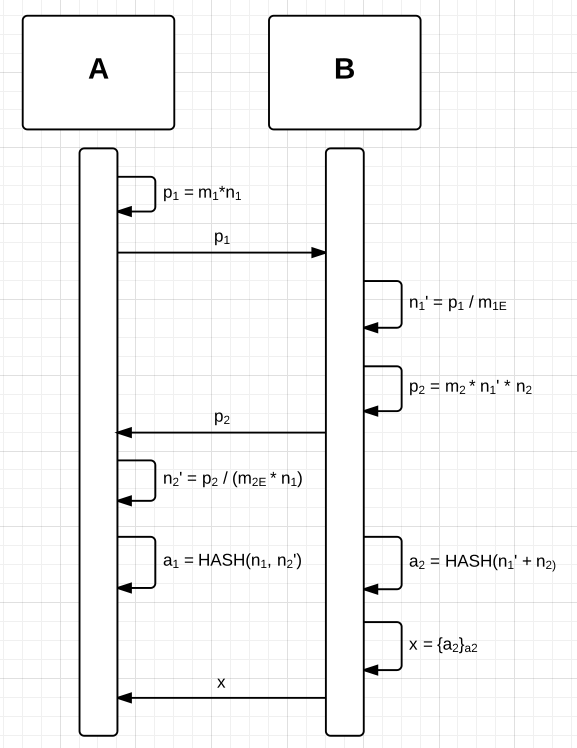
\includegraphics[height=150mm]{MeasurementDeadlockResolution.png}
\caption{Measurement Deadlock Resolution \label{overflow}}
\end{figure}

\begin{itemize}
\item The first message $A$ sends is $p_1$. Note that $A$ has not violated its privacy policy since $m_1$ is masked with a nonce. 
\item $B$ takes $p_1$ and makes a guess as to the value of $n_1$ based on $m_{1E}$. $m_{1E}$ is the ideal measurement which $B$ is expecting. Note that here we assume there is only 1 acceptable measurement value where in reality there may be a number of acceptable measurements. This protocol is easily extendable to handle such a case and is left as an exercise to the reader. However, it is worth noting that this has an appraiser side time complexity of $O(m * n^2)$ where $m$ is the number of acceptable measurements from $B$ and $n$ is the number of acceptable measurements from $A$.
\item $B$ then calculates a new value to send to $A$ that is $p_2 = m_2*n_1'*n_2$ where $n_2$ is a nonce generated by $B$
\item Note that when $B$ sends to $A$ the message $p_2$, $B$ has not violated its own privacy policy since the measurement $m_2$ is masked with nonce $n_2$
\item Now $A$ can make a guess as to the value of $n_2$ \textit{under the assumption $B$ was able to correctly guess $n_1$ (i.e. $B$ received the measurement $B$ was expecting)}
\item Now each entity computes a hash of their own nonce and the guess of the other's.
\item $B$ then sends $A$ $a_2$ encrypted or hashed with $a_2$
\item $A$ then compares $\{\{a_2\}_{a_2}\}_{a_1^{-1}}$ with $a_1$ (not shown).
\end{itemize}

So what does this give us? Note that neither party has broken their privacy policy. Additionally, note that $a_1 = a_2$ \textit{if and only if} both parties received the measurements they expected. Here is a short proof. 

We want to show that
\begin{center}
$a_1 = a_2$  iff $(m_1 = m_{1E}) \land (m_2 = m_{2E})$
\end{center}
Therfore we will show 
\begin{align*}
 (a_1 = a_2) \Longrightarrow (m_1 = m_{1E}) \land (m_2 = m_{2E})\\
 and \\
 (m_1 = m_{1E}) \land (m_2 = m_{2E}) \Longrightarrow (a_1 = a_2)
\end{align*}
\textbf{Proof of $ (m_1 = m_{1E}) \land (m_2 = m_{2E}) \Longrightarrow (a_1 = a_2)$:}\\
Recall $n_1' = \frac {m_1n_1} {m_{1E}}$. Therefore it is clear to see that if $m_1 = m_{1E}$, then $n_1 = n_1'$. \\
Similarly, recall $n_2' = \frac{m_2n_1'n_2}{(m_{2E})n_1}$. \\
We have already shown that $n_1 = n_1'$ and we are given that $m_2 = m_{2E}$.\\
Therefore it shows that $n_2 = n_2'$ and therefore the hashes of $(n_1,n_2') = (n_1',n_2)$\\

\textbf{Proof of $ (a_1 = a_2) \Longrightarrow (m_1 = m_{1E}) \land (m_2 = m_{2E})$:}\\
Note:\\
\begin{align*}
&a_1 = \#(n_1, n_2') &&a_2 = \#(n_1', n_2) \\
&a_1 = \#(n_1, \frac{p_2}{(m_{2E})n_1}) &&a_2 = \#(\frac{p_1}{m_{1E}}, n_2) \\
\\
&a_1 = \#(n_1, \frac{m_2n_1'n_2}{(m_{2E})n_1}) &&a_2 = \#(\frac{m_1n_1}{m_{1E}},  n_2)
\end{align*}
We are given $a_1 = a_2 $. That is,
\begin{align*}
\#(n_1, \frac{m_2n_1'n_2}{(m_{2E})n_1}) = \#(\frac{m_1n_1}{m_{1E}}, n_2)
\end{align*}
Note under our cryptographic assumption of hashes, that\\ 
since $a_1 = HASH(n_1,n_2')$ and $a_2 = HASH(n_1',n_2)$, then \\ 
$a_1 = a_2$ \textit{iff} $(n_1 = n_1') \land (n_2 = n_2')$
Therefore we know
\begin{align*}
n_1 = \frac{m_1n_1}{m_{1E}} && n_2 = \frac{m_2n_1'n_2}{(m_{2E})n_1}
\end{align*}
It shows that the only solution to the left side equation (assuming no 0 values) is when $m_1 = m_{1E}$.\\
Recall the implication derived previously: $(m_1 = m_{1E}) \Longrightarrow (n_1' = n_1)$. This gives us 
\begin{equation*}
n_2 = \frac{m_2n_2}{(m_{2E})}
\end{equation*}
Which is only true when $m_2 = m_{2E}$ (again assuming no 0 values).\\
Therefore,
\begin{equation}
a_1 = a_2 \Longleftrightarrow (m_1 = m_{1E}) \land (m_2 = m_{2E})
\end{equation}

Note that we do have a couple of requirements for this method of resolution.
\begin{enumerate}
\item Measurements must be non-zero
\item The nonces generated must not be restricted to integers. Otherwise information can be revealed ``too soon"--i.e. when $B$ calculates $n_1'$, $B$ would know correctness by checking if the division gives an integer solution or not. 
\end{enumerate} 













\begin{comment}
We also have some implications to keep in mind.

\begin{align*}
&(m_1 = m_{1E}) \Longrightarrow (n_1' = n_1),\\
&(m_2 = m_{2E}) \land (n_1 = n_1') \Longrightarrow (n_2' = n_2)\\
&(n_1 = n_1') \land (n_2 = n_2') \Longrightarrow (a_1 = a_2)\\
&that \quad is,\\
&(m_1 = m_{1E}) \land (m_2 = m_{2E}) \Longrightarrow (a_1 = a_2) 
\end{align*}
This is all well and good, but what we really want to show is
\begin{align*}
&(m_1 = m_{1E}) \land (m_2 = m_{2E}) \Longleftrightarrow (a_1 = a_2) 
\end{align*}
If $B$ does not get the measurement expected ($m_{1E}$) then $n_1' \neq n_1$. Then even if $m_{2E} = m_2$, $n_2' \neq n_2$. It follows that $a_1 \neq a_2$ and the decryption check will fail.   both parties abide by their privacy policy for one. either party has broken their privacy policy for one, and $n_1$.\\
Therefore 

\end{comment}



 
 
\end{document}